\documentclass[12pt,a4paper]{scrartcl} 
\usepackage[utf8]{inputenc}
\usepackage[english,russian]{babel}
\usepackage{indentfirst}
\usepackage{misccorr}
\usepackage{graphicx}
\usepackage{amsmath}
\usepackage{url}
\usepackage{float}
\usepackage{tikz}
\usetikzlibrary{shapes.geometric, arrows.meta, positioning, calc}

\graphicspath{{../Otchet/}}

\tikzset{
	block/.style={rectangle, draw, align=center, minimum width=3.4cm, minimum height=0.75cm},
	terminal/.style={rectangle, draw, rounded corners=10pt, align=center, minimum width=3.4cm, minimum height=0.75cm},
	decision/.style={diamond, draw, aspect=2, align=center, inner sep=3pt, minimum width=2.8cm},
	arr/.style={-{Stealth[length=2mm]}}
}

\newlength{\ML}

\begin{document}

\begin{titlepage}
	\begin{center}
		\large
		МИНИСТЕРСТВО НАУКИ И ВЫСШЕГО ОБРАЗОВАНИЯ РОССИЙСКОЙ ФЕДЕРАЦИИ
		
		Федеральное государственное бюджетное образовательное учреждение высшего образования
		
		\textbf{АДЫГЕЙСКИЙ ГОСУДАРСТВЕННЫЙ УНИВЕРСИТЕТ}
		\vspace{0.25cm}
		
		НОК "Институт точных наук и цифровых технологий"
		
		Кафедра автоматизированных систем обработки информации и управления
		\vfill
		\vfill
		
		\textsc{Отчет по ознакомительной практике}\\[5mm]
		
		{\LARGE Численные методы. \textit{Вариант 50}}
		\bigskip
		
		1 курс, группа 1ИВТ
	\end{center}
	\vfill
	
	\settowidth{\ML}{«\underline{\hspace{0.7cm}}» \underline{\hspace{2cm}}}
	\hfill\begin{minipage}{0.5\textwidth}
		Выполнил:\\
		\underline{\hspace{\ML}} Д.\,Б.~Самогов\\
		«\underline{\hspace{0.7cm}}» \underline{\hspace{2cm}} 2026 г.
	\end{minipage}%
	\bigskip
	
	\hfill\begin{minipage}{0.5\textwidth}
		Руководитель:\\
		\underline{\hspace{\ML}} С.\,В.~Теплоухов\\
		«\underline{\hspace{0.7cm}}» \underline{\hspace{2cm}} 2026 г.
	\end{minipage}%
	\vfill
	
	\begin{center}
		Майкоп, 2026 г.
	\end{center}
\end{titlepage}

\section{Введение}

\textbf{Номер варианта: 50.}

Цель работы --- программная реализация численных методов по методическим указаниям~\cite{Zadanie-2026}: решение трансцендентного уравнения $\sqrt{1-x}=5\sin x$, системы линейных уравнений методом Гаусса и расчёт эквивалентного сопротивления мостовой цепи (задача~2.10)~\cite{Uvarov-2000, Samarsky-1989, Trofimov-2015}.

Отчёт оформлен в \LaTeX{}~\cite{Lvovsky-2003}; программы написаны на языке Python~\cite{Python-2026} и содержат:
\begin{enumerate}
 \item номер варианта;
 \item исходные данные задач;
 \item ход решения с блок-схемами алгоритмов;
 \item интерпретацию результатов;
 \item выводы;
 \item программы на языке Python (фрагменты кода приведены в тексте, полные файлы --- в репозитории).
\end{enumerate}

%==============================================================================

\section{Лабораторная работа №1. Нелинейное уравнение}

\subsection{Исходные данные}

\begin{itemize}
 \item \textbf{Вариант:} 50.
 \item \textbf{Уравнение:} $\sqrt{1-x}=5\sin x$.
 \item \textbf{Методы:} бисекция отрезка и метод секущих~\cite{Uvarov-2000}.
 \item \textbf{Точность:} $\varepsilon = 0{,}01$.
 \item \textbf{Язык программирования:} Python, файл \texttt{Program/lab1\_nonlinear.py}.
\end{itemize}

\subsection{Ход решения}

\textbf{Шаг 1.} Задаём $f(x)=\sqrt{1-x}-5\sin x$ и отделяем корни на сетке $x\le 1$: ищем интервалы $[a;b]$, где $f(a)\cdot f(b)<0$.

\textbf{Шаг 2.} На каждом интервале находим корень методом бисекции и методом секущих.

\textbf{Шаг 3.} Сравниваем результаты и проверяем $|f(x)|<\varepsilon$.

\textbf{Фрагмент программы} (файл \texttt{Program/lab1\_nonlinear.py}):
\begin{verbatim}
def f(x):
    if x > 1.0:
        return float("nan")
    return math.sqrt(1.0 - x) - 5.0 * math.sin(x)

def bisection(func, left, right, eps=0.01):
    while right - left > eps:
        middle = (left + right) / 2
        if func(left) * func(middle) <= 0:
            right = middle
        else:
            left = middle
    return (left + right) / 2

def secant(func, x0, x1, eps=0.01):
    while True:
        f0, f1 = func(x0), func(x1)
        if abs(f1) < eps:
            return x1
        x2 = x1 - f1 * (x1 - x0) / (f1 - f0)
        if abs(x2 - x1) < eps:
            return x2
        x0, x1 = x1, x2
\end{verbatim}

\subsubsection{Блок-схемы алгоритмов}

Блок-схема метода бисекции --- рис.~\ref{fig:flow-bisect}. Блок-схема общего алгоритма программы --- рис.~\ref{fig:flow-lab1}.

\begin{figure}[H]
	\centering
    \begin{tikzpicture}[
        scale=0.78, transform shape,
        block/.style={rectangle, draw, rounded corners=2pt, align=center, minimum width=3.2cm, minimum height=0.7cm},
        terminal/.style={rectangle, draw, rounded corners=10pt, align=center, minimum width=3.2cm, minimum height=0.7cm},
        decision/.style={diamond, draw, aspect=2, align=center, inner sep=3pt, minimum width=2.6cm},
        arr/.style={-{Stealth[length=2mm]}}
    ]
        \node[terminal] (start) at (0, 0) {Начало};
        \node[block] (in) at (0, -1.6) {Ввод $a$, $b$, $\varepsilon$};
        \node[decision] (dec) at (0, -3.6) {$b-a>\varepsilon$?};
        \node[block] (mid) at (0, -5.4) {$c=(a+b)/2$};
        \node[decision] (dec2) at (0, -7.2) {$f(a)f(c)\le 0$?};
        \node[block] (bset) at (-3.4, -9.0) {$b:=c$};
        \node[block] (aset) at (3.4, -9.0) {$a:=c$};
        \node[block] (out) at (-5.8, -3.6) {$x=(a+b)/2$};
        \node[terminal] (stop) at (-5.8, -5.4) {Конец};

        \coordinate (merge) at (5.8, -10.2);

        \draw[arr] (start) -- (in);
        \draw[arr] (in) -- (dec);
        \draw[arr] (dec) -- node[right, scale=0.85] {да} (mid);
        \draw[arr] (mid) -- (dec2);
        \draw[arr] (dec2.west) -| node[above, pos=0.25, scale=0.85] {да} (bset.north);
        \draw[arr] (dec2.east) -| node[above, pos=0.25, scale=0.85] {нет} (aset.north);
        \draw (bset.south) -- (bset.south |- merge);
        \draw (aset.south) -- (aset.south |- merge);
        \draw (aset.south |- merge) -- (merge);
        \draw[arr] (merge) -- (merge |- dec.east) -- (dec.east);

        \draw[arr] (dec.west) -- node[above, scale=0.85] {нет} (out.east);
        \draw[arr] (out) -- (stop);
    \end{tikzpicture}
    \caption{Блок-схема метода бисекции}\label{fig:flow-bisect}
\end{figure}

\begin{figure}[H]
	\centering
    \resizebox{\textwidth}{!}{%
    \begin{tikzpicture}[
        scale=0.78, transform shape,
        block/.style={rectangle, draw, rounded corners=2pt, align=center, minimum width=3.5cm, minimum height=0.7cm},
        terminal/.style={rectangle, draw, rounded corners=10pt, align=center, minimum width=3.5cm, minimum height=0.7cm},
        decision/.style={diamond, draw, aspect=2, align=center, inner sep=3pt, minimum width=2.8cm},
        arr/.style={-{Stealth[length=2mm]}}
    ]
        \node[terminal] (start) at (0, 0) {Начало};
        \node[block] (func) at (3.8, 0) {$f(x)=\sqrt{1-x}-5\sin x$};
        \node[block] (scan) at (7.6, 0) {Сканирование $[-10;1]$};
        \node[decision] (found) at (11.4, 0) {Есть\\интервалы?};
        \node[block] (bis) at (15.2, 0) {Бисекция};
        \node[block] (sec) at (19.0, 0) {Секущие};
        \node[decision] (more) at (22.8, 0) {Ещё\\интервалы?};
        \node[block] (save) at (26.6, 0) {График и скриншот};
        \node[terminal] (stop) at (30.4, 0) {Конец};
        \node[block] (empty) at (11.4, -2.4) {Сообщение};

        \coordinate (loopback) at (15.2, -2.4);

        \draw[arr] (start) -- (func);
        \draw[arr] (func) -- (scan);
        \draw[arr] (scan) -- (found);
        \draw[arr] (found) -- node[above, scale=0.85] {да} (bis);
        \draw[arr] (bis) -- (sec);
        \draw[arr] (sec) -- (more);
        \draw[arr] (more) -- node[above, scale=0.85] {нет} (save);
        \draw[arr] (save) -- (stop);

        \draw[arr] (found.south) -- node[right, scale=0.85] {нет} (empty.north);
        \draw[arr] (empty.south) -- ++(0,-0.8) -| (stop.south);

        \draw[arr] (more.south) -- ++(0,-0.5) -| node[near start, right, scale=0.85] {да} (loopback);
        \draw[arr] (loopback) -- (bis.south);
    \end{tikzpicture}
    }
    \caption{Блок-схема программы ЛР №1}\label{fig:flow-lab1}
\end{figure}

\subsection{Результаты}

График функции и отделённые корни --- рис.~\ref{fig:lab1plot}. Найдены три корня на интервале $[-10;1]$:
\begin{itemize}
 \item $x\approx -5{,}72$;
 \item $x\approx -3{,}57$;
 \item $x\approx 0{,}18$.
\end{itemize}

\begin{figure}[H]
	\centering
	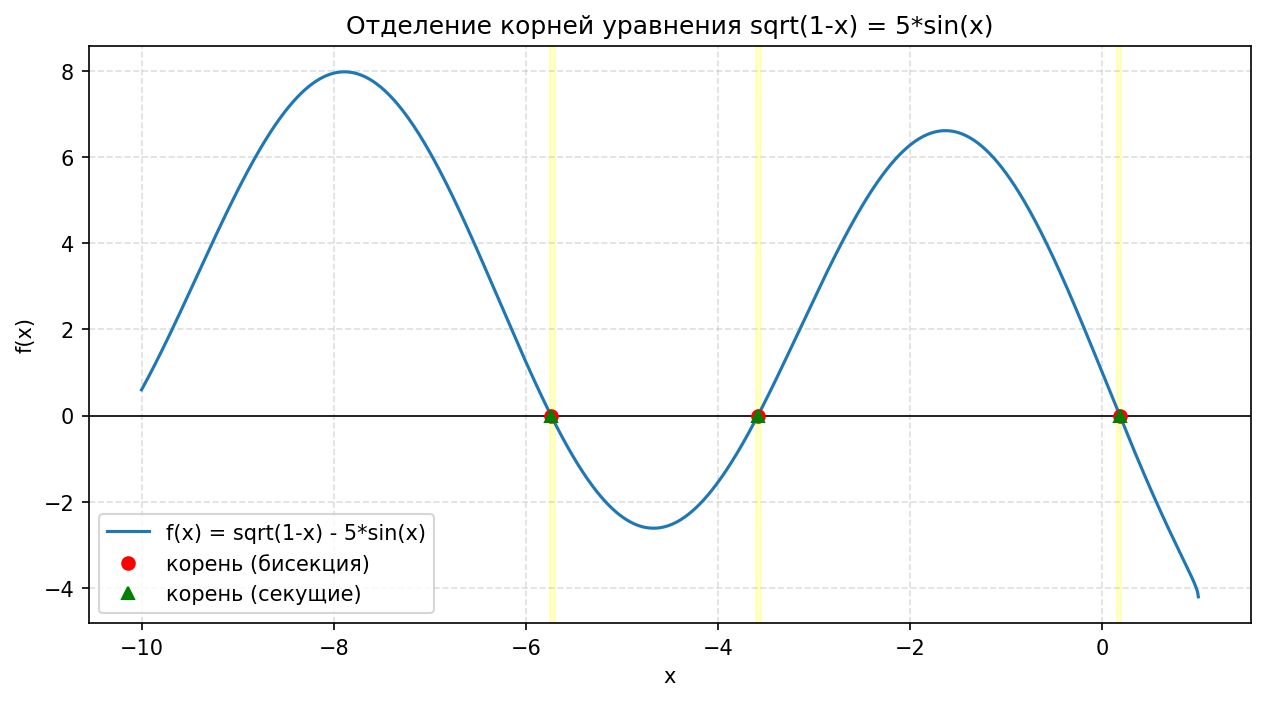
\includegraphics[width=0.95\textwidth]{lab1_plot.png}
	\caption{График $f(x)=\sqrt{1-x}-5\sin x$ и локализация корней}\label{fig:lab1plot}
\end{figure}

\begin{figure}[H]
	\centering
	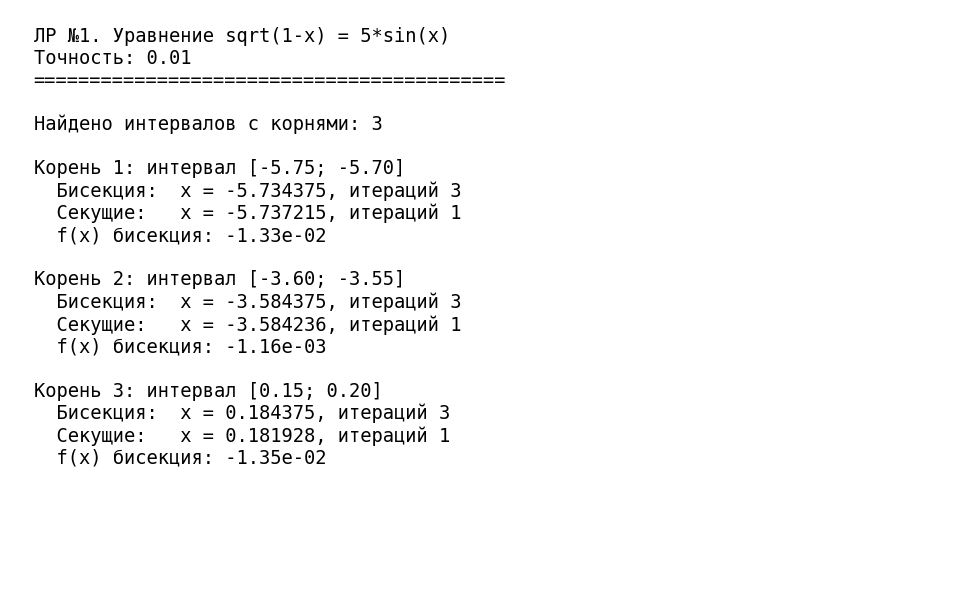
\includegraphics[width=0.75\textwidth]{lab1_output.png}
	\caption{Вывод программы ЛР №1}\label{fig:lab1out}
\end{figure}

\subsection{Интерпретация результатов}

Найденные значения $x$ --- точки пересечения графика $y=\sqrt{1-x}$ с $y=5\sin x$. При $x\le 1$ подкоренное выражение неотрицательно. Корни около $-5{,}7$, $-3{,}6$ и $0{,}2$ соответствуют трём участкам смены знака функции. Оба метода дают совпадающие результаты с точностью $0{,}01$.

\subsection{Выводы по ЛР №1}

Реализованы отделение корней, метод бисекции и метод секущих. Программа находит корни уравнения $\sqrt{1-x}=5\sin x$ с требуемой точностью; результаты подтверждены графиком и вычислением $f(x)$.

%==============================================================================

\section{Лабораторная работа №2. Система линейных уравнений}

\subsection{Исходные данные}

\begin{itemize}
 \item \textbf{Вариант:} 50.
 \item \textbf{Метод:} Гаусса~\cite{Samarsky-1989}.
 \item \textbf{Точность:} $0{,}01$.
 \item \textbf{Матрица $A$ и вектор $\mathbf{b}$:}
\[
A=\begin{pmatrix}
0{,}78 & -0{,}02 & -0{,}12\\
0{,}02 & -0{,}86 & 0{,}04\\
0{,}12 & 0{,}44 & -0{,}72
\end{pmatrix},
\quad
\mathbf{b}=\begin{pmatrix}-0{,}56\\ 0{,}77\\ 1{,}01\end{pmatrix}.
\]
 \item \textbf{Программа:} \texttt{Program/gauss.py}.
\end{itemize}

\subsection{Ход решения}

\textbf{Шаг 1.} Формируется расширенная матрица $[A|\mathbf{b}]$.

\textbf{Шаг 2.} Прямой ход: выбор главного элемента, обнуление элементов под диагональю.

\textbf{Шаг 3.} Обратный ход: вычисление $x_n, x_{n-1}, \ldots, x_1$.

\textbf{Шаг 4.} Проверка невязок $A\mathbf{x}-\mathbf{b}$.

\textbf{Фрагмент программы} (файл \texttt{Program/gauss.py}):
\begin{verbatim}
def gauss_solve(matrix, vector):
    validate_system(matrix, vector)
    n = len(vector)
    augmented = copy_augmented(matrix, vector)

    rank = 0
    for column in range(n):
        pivot_row = find_pivot(augmented, column, rank)
        if pivot_row is None:
            continue
        # перестановка строк и обнуление столбца
        ...
        rank += 1

    solution = [0.0] * n
    for row in range(n - 1, -1, -1):
        value = augmented[row][n]
        for col in range(row + 1, n):
            value -= augmented[row][col] * solution[col]
        solution[row] = value / augmented[row][row]
    return solution
\end{verbatim}

\subsubsection{Блок-схема алгоритма}

Блок-схема метода Гаусса --- рис.~\ref{fig:flow-gauss}.

\begin{figure}[H]
	\centering
    \begin{tikzpicture}[
        scale=0.76, transform shape,
        block/.style={rectangle, draw, rounded corners=2pt, align=center, minimum width=3.3cm, minimum height=0.7cm},
        terminal/.style={rectangle, draw, rounded corners=10pt, align=center, minimum width=3.3cm, minimum height=0.7cm},
        decision/.style={diamond, draw, aspect=2, align=center, inner sep=3pt, minimum width=2.6cm},
        arr/.style={-{Stealth[length=2mm]}}
    ]
        \node[terminal] (start) at (0, 0) {Начало};
        \node[block] (in) at (0, -1.6) {Ввод $A$, $\mathbf{b}$};
        \node[decision] (ok) at (0, -3.6) {Данные\\корректны?};
        \node[block] (aug) at (0, -5.6) {$[A|\mathbf{b}]$};
        \node[block] (kinit) at (0, -7.2) {$k:=1$};
        \node[decision] (fwd) at (0, -9.2) {$k\le n$?};

        \node[block] (pivot) at (4.8, -9.2) {Главный\\элемент};
        \node[block] (zero) at (4.8, -10.8) {Обнулить\\столбец $k$};
        \node[block] (inc) at (4.8, -12.4) {$k:=k+1$};

        \node[block] (iinit) at (0, -11.2) {$i:=n$};
        \node[decision] (back) at (0, -13.2) {$i\ge 1$?};
        \node[block] (xi) at (-4.8, -13.2) {Найти $x_i$};
        \node[block] (idec) at (-4.8, -14.8) {$i:=i-1$};

        \node[block] (check) at (0, -15.6) {Проверка $A\mathbf{x}-\mathbf{b}$};
        \node[block] (out) at (0, -17.2) {Вывод $\mathbf{x}$};
        \node[terminal] (stop) at (0, -18.8) {Конец};
        \node[block] (err) at (4.8, -3.6) {Ошибка};

        \coordinate (fwd-loop) at (7.0, -12.4);
        \coordinate (back-loop) at (-7.0, -15.4);

        \draw[arr] (start) -- (in);
        \draw[arr] (in) -- (ok);
        \draw[arr] (ok) -- node[right, scale=0.85] {да} (aug);
        \draw[arr] (aug) -- (kinit);
        \draw[arr] (kinit) -- (fwd);

        \draw[arr] (ok.east) -- node[above, scale=0.85] {нет} (err.west);
        \draw[arr] (err.south) -- ++(0,-8.0) -| (stop.east);

        \draw[arr] (fwd.east) -- node[above, scale=0.85] {да} (pivot.west);
        \draw[arr] (pivot) -- (zero);
        \draw[arr] (zero) -- (inc);
        \draw[-] (inc.east) -- (fwd-loop);
        \draw[arr] (fwd-loop) |- (fwd.south);

        \draw[arr] (fwd) -- node[right, scale=0.85] {нет} (iinit);
        \draw[arr] (iinit) -- (back);
        \draw[arr] (back.west) -- node[above, scale=0.85] {да} (xi.east);
        \draw[arr] (xi) -- (idec);
        \draw[-] (idec.south) -- ++(0,-0.6) -| (back-loop);
        \draw[arr] (back-loop) |- (back.west);

        \draw[arr] (back) -- node[right, scale=0.85] {нет} (check);
        \draw[arr] (check) -- (out);
        \draw[arr] (out) -- (stop);
    \end{tikzpicture}
    \caption{Блок-схема метода Гаусса}\label{fig:flow-gauss}
\end{figure}

\subsection{Результаты}

\[
x_1\approx -1{,}08,\quad x_2\approx -1{,}02,\quad x_3\approx -2{,}21.
\]

Невязки $\approx 10^{-16}$. График и вывод программы --- рис.~\ref{fig:gaussplot}, \ref{fig:gaussout}.

\begin{figure}[H]
	\centering
	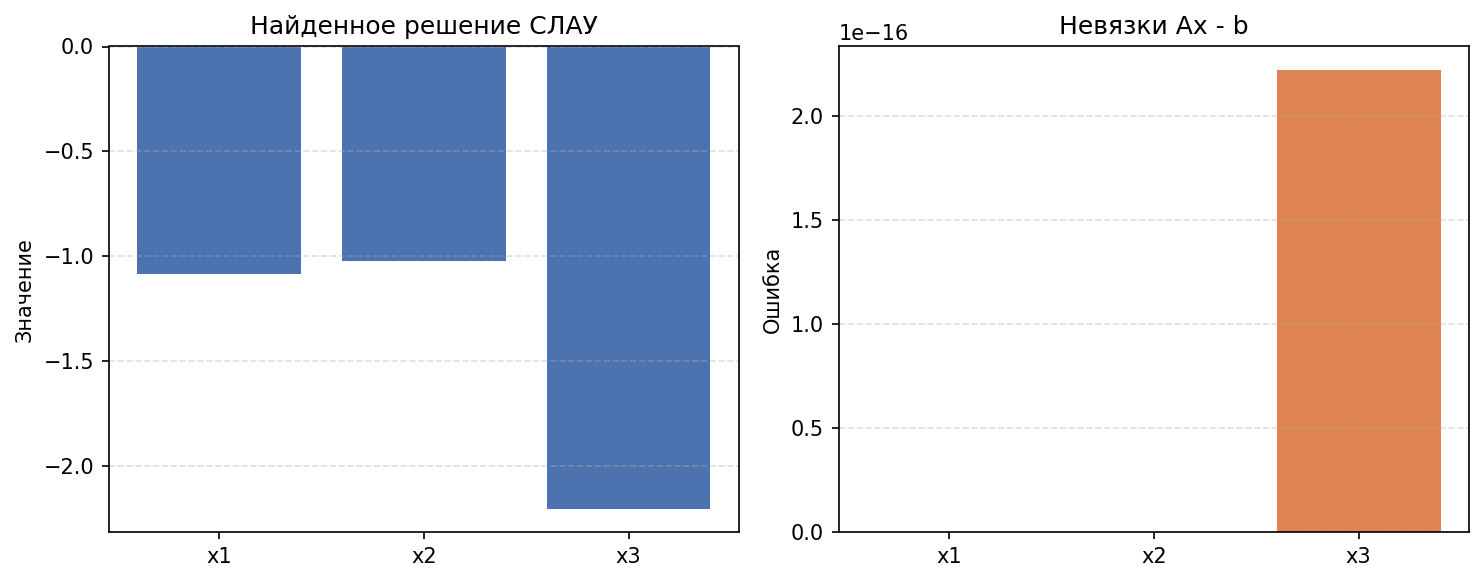
\includegraphics[width=0.9\textwidth]{gauss_solution.png}
	\caption{Решение СЛАУ варианта 50}\label{fig:gaussplot}
\end{figure}

\begin{figure}[H]
	\centering
	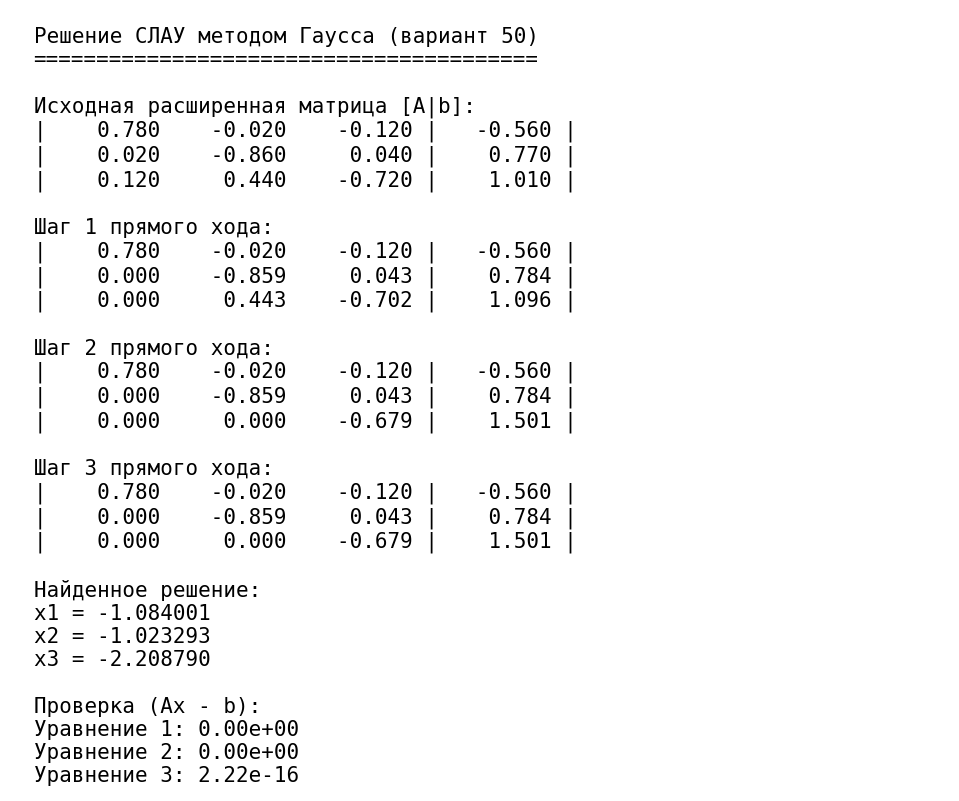
\includegraphics[width=0.85\textwidth]{gauss_output.png}
	\caption{Вывод программы метода Гаусса}\label{fig:gaussout}
\end{figure}

\subsection{Интерпретация результатов}

Вектор $\mathbf{x}$ --- набор неизвестных системы трёх линейных уравнений. Все три компоненты отрицательны: $x_1\approx -1{,}08$, $x_2\approx -1{,}02$, $x_3\approx -2{,}21$. Малые невязки подтверждают, что найденный вектор удовлетворяет исходной системе $A\mathbf{x}=\mathbf{b}$.

\subsection{Выводы по ЛР №2 (задание 1)}

Метод Гаусса реализован с проверкой входных данных и выбором главного элемента. Система варианта~50 имеет единственное решение, найденное с высокой точностью.

%==============================================================================

\section{Лабораторная работа №2. Задание 2.10}

\subsection{Исходные данные}

\begin{itemize}
 \item \textbf{Задача:} 2.10.
 \item Найти сопротивление цепи между точками $A$ и $B$.
 \item $R=120$~Ом (в схеме используются также $R/2$ и перемычка $R$).
 \item \textbf{Программа:} \texttt{Program/lab2\_resistance.py}.
\end{itemize}

\subsection{Ход решения}

Цепь --- мост между точками $A$ и $B$: верхняя ветвь $R$ и $R/2$, нижняя $R/2$ и $R$, между серединами перемычка $R$~\cite{Trofimov-2015}. Применяется узловой метод: задаём $V_A=1$, $V_B=0$, находим потенциалы внутренних узлов и ток из $A$.

\[
R_{AB}=\frac{U_{AB}}{I_A}\approx 85{,}71~\text{Ом}.
\]

Без перемычки получилось бы $R\approx 90$~Ом.

\textbf{Фрагмент программы} (файл \texttt{Program/lab2\_resistance.py}):
\begin{verbatim}
R = 120.0

def solve_resistance_210(base_r=R):
    r_tl = base_r
    r_tr = base_r / 2.0
    r_bl = base_r / 2.0
    r_br = base_r
    r_bridge = base_r
    # узловой метод, V_A=1, V_B=0
    ...
    return {"R_AB": 1.0 / current_from_a}
\end{verbatim}

\subsubsection{Блок-схема алгоритма}

Блок-схема программы --- рис.~\ref{fig:flow-circuit}.

\begin{figure}[H]
	\centering
    \resizebox{\textwidth}{!}{%
    \begin{tikzpicture}[
        scale=0.78, transform shape,
        block/.style={rectangle, draw, rounded corners=2pt, align=center, minimum width=3.4cm, minimum height=0.7cm},
        terminal/.style={rectangle, draw, rounded corners=10pt, align=center, minimum width=3.4cm, minimum height=0.7cm},
        decision/.style={diamond, draw, aspect=2, align=center, inner sep=3pt, minimum width=2.8cm},
        arr/.style={-{Stealth[length=2mm]}}
    ]
        \node[terminal] (start) at (0, 0) {Начало};
        \node[block] (data) at (3.8, 0) {$R=120$~Ом};
        \node[block] (g) at (7.6, 0) {Матрица\\проводимостей};
        \node[decision] (det) at (11.4, 0) {$\det\neq 0$?};
        \node[block] (v) at (15.2, 0) {$V_T$, $V_D$};
        \node[block] (i) at (19.0, 0) {$I_A$};
        \node[block] (req) at (22.8, 0) {$R_{AB}=1/I_A$};
        \node[block] (out) at (26.6, 0) {Вывод};
        \node[terminal] (stop) at (30.4, 0) {Конец};
        \node[block] (err) at (11.4, -2.4) {Ошибка};

        \draw[arr] (start) -- (data);
        \draw[arr] (data) -- (g);
        \draw[arr] (g) -- (det);
        \draw[arr] (det) -- node[above, scale=0.85] {да} (v);
        \draw[arr] (v) -- (i);
        \draw[arr] (i) -- (req);
        \draw[arr] (req) -- (out);
        \draw[arr] (out) -- (stop);

        \draw[arr] (det.south) -- node[right, scale=0.85] {нет} (err.north);
        \draw[arr] (err.south) -- ++(0,-0.8) -| (stop.south);
    \end{tikzpicture}
    }
    \caption{Блок-схема программы задачи 2.10}\label{fig:flow-circuit}
\end{figure}

\subsection{Результаты}

$R_{AB}\approx 85{,}71$~Ом. Скриншот --- рис.~\ref{fig:circuit}.

\begin{figure}[H]
	\centering
	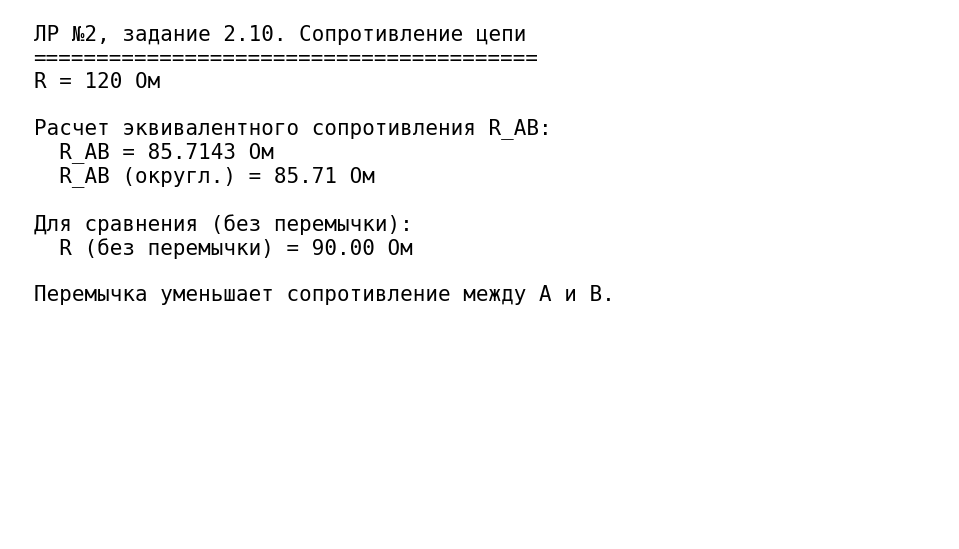
\includegraphics[width=0.85\textwidth]{lab2_resistance_output.png}
	\caption{Вывод программы задачи 2.10}\label{fig:circuit}
\end{figure}

\subsection{Интерпретация результатов}

Эквивалентное сопротивление $85{,}7$~Ом меньше, чем при отсутствии перемычки ($90$~Ом): дополнительный путь через мостовую перемычку $R$ снижает общее сопротивление между $A$ и $B$.

\subsection{Выводы по заданию 2.10}

Задача 2.10 решена узловым методом и проверена программой. Сопротивление цепи между точками $A$ и $B$ равно $85{,}71$~Ом.

%==============================================================================

\section{Общие выводы}

\begin{enumerate}
 \item Выполнены все задания \textbf{варианта 50}: нелинейное уравнение, СЛАУ методом Гаусса, расчёт сопротивления цепи (задача 2.10).
 \item Составлены программы на Python с контролем входных данных (файлы \texttt{lab1\_nonlinear.py}, \texttt{gauss.py}, \texttt{lab2\_resistance.py}).
 \item Построены блок-схемы алгоритмов (рис.~\ref{fig:flow-bisect}--\ref{fig:flow-circuit}).
 \item Результаты интерпретированы в терминах исходных задач и подтверждены графиками и проверками.
\end{enumerate}


\section{Список литературы}

\begin{thebibliography}{9}
\bibitem{Zadanie-2026}Методические указания по ознакомительной практике «Численные методы». Вариант~50. Файл \texttt{zadanie.pdf}.
\bibitem{Uvarov-2000}Уваров, С. Математические методы физики / С.\,К.~Уваров, Е.\,Б.~Барулин, И.\,Л.~Розенталь. --- М.: Атомиздат, 2000. --- Гл.~о методах решения нелинейных уравнений (бисекция, секущие).
\bibitem{Samarsky-1989}Самарский, А. Численные методы / А.\,А.~Самарский, А.\,В.~Гулин. --- 2-е изд. --- М.: Наука, 1989. --- Гл.~о методе Гаусса для СЛАУ.
\bibitem{Trofimov-2015}Трофимова, Т. Курс общей физики. Электричество и магнетизм / Т.\,И.~Трофимова. --- М.: Академия, 2015. --- Законы Кирхгофа, расчёт цепей постоянного тока.
\bibitem{Kalashnikov-2004}Калашников, С. Общая физика. Т.~2. Электричество и магнетизм / С.\,Г.~Калашников. --- М.: Физматлит, 2004. --- Эквивалентное сопротивление разветвлённых цепей.
\bibitem{Python-2026}Документация Python~3 [Электронный ресурс]. URL: \url{https://docs.python.org/3/} (дата обращения: 21.06.2026).
\bibitem{Matplotlib-2026}Matplotlib: Visualization with Python [Электронный ресурс]. URL: \url{https://matplotlib.org/} (дата обращения: 21.06.2026).
\bibitem{Lvovsky-2003}Львовский, С. Набор и верстка в системе \LaTeX{} / С.\,М.~Львовский. --- 3-е изд. --- М.: Академический проект, 2003.
\end{thebibliography}

\end{document}